\documentclass{article}
\usepackage[utf8]{inputenc}
\usepackage{authblk}
\usepackage{graphicx}


\title{Tip Toe: Reinforcement Learning for Robotic Operations with Input Constraints}

\author{Tammer Barkouki}
\author{Diego Rojas}
\author{Thomas Matthews}
\affil{}

\date{\today}

\begin{document}

\maketitle

\newpage

\section{Overview}
We aim to use reinforcement learning to control a three-armed robot which minimizes the force applied to the arms the robot is standing on when pushing an object or moving. The motivating use-cases for this research are autonomous robots for search and rescue \cite{jacoff2001standard}, mobile robotic telesurgery \cite{lum2007telesurgery} and intravehicular robotics in future deep space habitats such as NASA's Gateway \cite{coderre2019concept}. All three applications present mobility challenges due to uncertainties in the environment. In the case of search and rescue, the robotic system may need to move in such a way that a minimum amount of force must be applied to one or more legs due to structural instability, as determined by perception using on-board sensors. In telesurgery, there may not be known infrastructure as in an operating room on which to affix the robot, so it may need to support itself in an unknown environment. In a space habitat, the robot may be deployed in unforeseen ways that require fastening itself to objects not rated as "handrails", in which case the amount of force/torque applied through the arms may be limited. In all cases, the robot will need a control policy that is not able to be explicitly engineered, and this motivates our exploration of adaptive optimal control and reinforcement learning \cite{sutton1992reinforcement}.

Initially to develop a control policy for the three-armed robot, we will utilize the OpenAI Gym platform \cite{brockman2016openai}. OpenAI Gym is a toolkit that provides benchmark environments for researchers to develop and train RL agents. The environment sets the system dynamics (e.g physics) in which the agent operates and rewards the agent for achieving the desired results. These rewards help the agent learn the policy (what actions to take in each state). For a three-armed robot, this means the environment provides the dynamics model, i.e. the equations of motion, the reaction forces of stationary surfaces resulting from the robot's weight and the forces and torques transmitted through the arms due to control inputs. The policy maps states, consisting of the positions and velocities of the robot's joints and objects it is interacting with, to actions, which are the joint control inputs.

Our initial application will be a two-armed robot operating in a 2-dimensional environment. After evaluating the two-armed robot and learning about the important tuning parameters needed to learn a policy, we will modify the our 2-dimensional environment to contain a three-armed robot. Finally, if time allows, we will explore creating a 3-dimensional environment for the three-armed robot to interact with.


%%%%%%%%%% old notes for Overview section:  %%%%%%%%%

%%% Problem motivated 3-legged robot concept for Gateway
%%% Interested in the dynamics of crawling/walking.
%%% Specifically, minimizing forces imparted on the environment
%%% Maximizing the transmission of force for, e.g. pushing or moving an object.
%%% Other applications in humanitarian search and rescue, such as in a collapsed structure where %%% minimizing the force on unstable surfaces may be necessary, as well as moving heavy debris.
%%% 
%%% Field Deploy-able operating table for disaster relief efforts. 
%%% 
%%% Demonstrations will occur in simulated environments.
%%% 
%%% Reinforcement Learning will be applied, leveraging OpenAI Gym.
%%% 
%%% Simple 2D case:
%%% 
%%% Harder 2D case (three arms?)
%%% 
%%% Hardest 3D case (3+ arms)

\section{Literature Review}
%% RL general lit review
Reinforcement learning (RL) is learning what actions to take given a situation in order to maximize some reward \cite{sutton2018reinforcement}. An \textbf{RL problem} formalizes the process of a goal-seeking \emph{agent} making decisions in a given \emph{state} to take an \emph{action} that maximizes a \emph{reward} it receives from its \emph{environment}.  An \textbf{RL algorithm} (aka solution method) is the computational analysis that solves the RL problem. The \textbf{field of RL} is the study of both the problems and solutions methods that apply RL. Our literature review will cover aspects of each of these: the field of RL, RL problems, and RL algorithms, thus we intend for the literature review of our final report will have the following subsections:

\subsection{RL basics and landscape of RL algorithm taxonomy}
Generally speaking, the advantage of RL over classical optimal control solutions is that RL algorithms do not need complete formulation of the system dynamics, meaning they cope better with uncertainties and allow for optimal control in adaptive autonomy. Our literature review will provide for an understanding of current research trends in RL algorithm development, and will leverage survey papers such as \cite{kiumarsi2017optimal} for comprehensive discussion of the RL algorithm landscape, as well as compiled lists of important papers for individual RL algorithms, e.g. \cite{key}.


\subsection{RL applied to robotic problems}
Following a general overview of RL, the literature review will focus on RL applied to robotic problems. This will help with formulating our problem in an RL sense, i.e. answering the "what are we learning?" question, such as a policy or a value function. Then we will focus on literature that sheds lights on how to select and tune an RL algorithm (or test a family of algorithms).

\subsection{Simulation technologies in training RL agents}
Due to the nature of RL problems requiring many training iterations, simulation environments are often leveraged for accelerated training. Simulations can run magnitudes faster than real time, can be ran in parallel, and therefore can obtain years worth of agent experience in a matter of days \cite{kadian2019we}. A literature review in this area will inform us on the different simulation tools and techniques used for training RL agents in simulation, as well as methods for generating a RL environment from scratch. 

\subsection{Transfer of RL policies from simulation to real world}
Three-dimensional physics based simulators are highly used to accelerate the training robots, with the intention to then transfer the trained policy to a real robot. However issues arise when transferring the RL policy from simulation to the real world due to the reality gap between simulation and real world. This sim2real transfer gap is often minimized by enhancing the physics of the simulators and including randomization in simulation. For example,  \cite{tan2018sim} focuses on training robust controllers for a Quadruped robot by randomizing dynamic parameters and adding random perturbations. Our literature review in this area will focus on understanding the different issues in transferring a RL policy from simulation to reality, and use this intuition to explain our results in the simulated environment.  




%% Search Terms
%RL for robotic manipulators \\
%Simulation Environments \\
%openAI \\
%Model Based RL


\section{Timeline and Contributions}

\subsection{Contributions:}
The learning objective for this project is for each student to gain an understanding of reinforcement learning and gain experience in modeling environments for reinforcement learning problems. Each student brings a different strength that is applicable for this project, and will lead certain aspects of the project based on strengths. Due to the similarity of our backgrounds every member will be involved to some degree with all of the different aspects of this project. We decided to allocate different tasks to each team member to give each of us a clear focus.

\begin{itemize}
    \item Tammer - Reinforcement learning in practice
        \begin{itemize}
            \item Investigate different reinforcement learning algorithms
            \item Tuning algorithm parameters
            \item Literature review: Reinforcement learning methods and policy optimization
        \end{itemize}
    \item Thomas - Dynamics model of the robot 
        \begin{itemize}
            \item 2D/3D Dynamic and kinematic models using Newton-Euler 
            \item Identify state vector for 2D/3D case
            \item Literature review: Model-based reinforcement learning
        \end{itemize}
    \item Diego - Reinforcement learning environment and simulation  
        \begin{itemize} 
            \item Define action and observation space
            \item Create reward system 2D/3D case
            \item Create simulation for 3D case
            \item Literature review: Simulation environments for RL
        \end{itemize}
\end{itemize}

\subsection{Timeline:} 
\begin{figure}[htp]
    \centering
    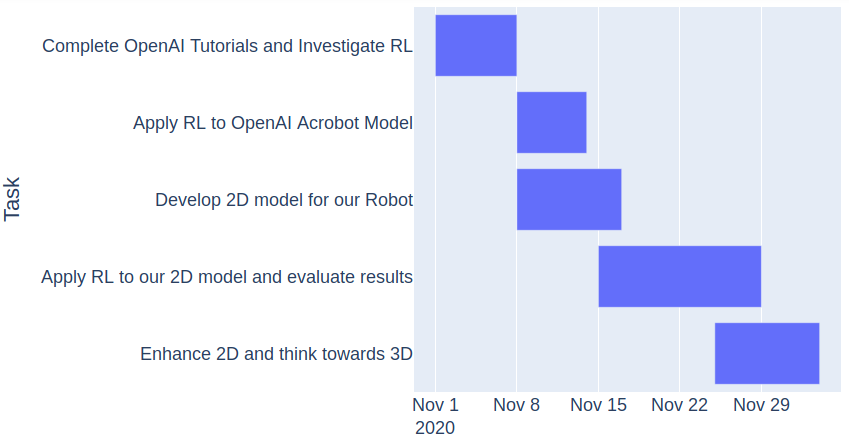
\includegraphics[width=10cm]{Project_timeline.png}
    \caption{The projected timeline}
    \label{fig:timeline}
\end{figure}
We will focus our efforts initially on completing the OpenAI tutorials and familiarizing ourselves with reinforcement learning. After which, we will solidify our understanding by applying reinforcement learning to the Acrobot environment \cite{acrobot}. As we are working on Acrobot, we will begin creating our own models for the two armed and three armed robots to be used. With a model in hand, we will then create an environment and reward policy and begin training the agent. Finally we will evaluate the results and attempt to repeat the process for a three dimensional robot if time allows. A week by week breakdown of the efforts is listed below:\\
\begin{itemize}
    \item Week 5% - Complete OpenAI tutorials and investigate Reinforcement Learning
    \begin{itemize}
        \item Complete OpenAI tutorials and investigate reinforcement learning.
    \end{itemize}
    \item Week 6 %- Apply Reinforcement Learning to the Acrobot OpenAI model
    \begin{itemize}
        \item Apply reinforcement learning to the Acrobot OpenAI model.
        \item Develop a 2D dynamic model for two armed robot.
    \end{itemize}
    \item Week 7% - Develop a 2D Dynamic Model for our robot and create environment
    \begin{itemize}
        \item Define reinforcement learning method to be used.
        \item Develop a 2D dynamic model for three armed robot.
        \item Create simulation environment and reward policy.
    \end{itemize}
    \item Week 8 %- Apply Reinforcement Learning to our 2-D model and evaluate results
    \begin{itemize}
        \item Begin testing of the two dimensional two armed robot.
    \end{itemize}
    \item Week 9% - Enhance 2D model and think towards 3D
    \begin{itemize}
        \item Review results and make any needed adjusts to model or environment.
        \item Create three dimensional model for three armed robot (if time allows).
        \item Create three dimensional simulation environment(if time allows).
    \end{itemize}
    \item Week 10% - Finalize results and prepare presentation
    \begin{itemize}
        \item Collect final results.
        \item Compile report.
        \item Create presentation of results.
    \end{itemize}
\end{itemize}

\bibliographystyle{IEEEtran}
\bibliography{references.bib}

\end{document}
